\section{LoRa}\label{sec:etat_art-lora}
\renewcommand{\rightmark}{LoRa}

LoRa (Long Range) est une technologie radio  fonctionnant sur une modulation radio propriétaire
détenue par Semtech. Cette modulation est dérive de la modulation \textit{chirp spread spectrum (CSS)} et permet d'obtenir des communications longues portées\todo{chiffres} et basses énergie.

Une communication LoRa dépend des paramètres suivants:
\begin{itemize}
    \item Spreading Factor (SF)
    \item Bandwidth (BW)
    \item Coding rate (CR)
\end{itemize}


%Le format des paquets LoRa est illustré à la figure~\ref{fig:state-lora-frame-format}. 
Le format des paquets LoRa(Fig.~\ref{fig:state-lora-frame-format}) peut être explicite ou implicite.
Dans le mode implicite, le header n'est pas inclus dans le paquet. Pour cela, la taille de la payload, le coding rate et la présence de la Payload CRC doit être configuré 
Ce mode permet de réduire la taille du paquet et donc du temps de transmission.

\begin{figure}[H]
    \centering
    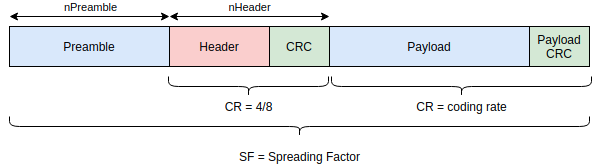
\includegraphics[scale=0.6]{res/pictures/lora-frame-format.drawio.png}
    \caption{Format d'un paquet LoRa.}
    \label{fig:state-lora-frame-format}
\end{figure}
